\documentclass[10pt,letterpaper,twocolumn]{article}
\usepackage[utf8]{inputenc}
\usepackage[spanish,es-tabla]{babel}
\decimalpoint
\let\cleardoublepage\clearpage
% \usepackage[bitstream-charter]{mathdesign}
% \usepackage[T1]{fontenc}
% \newcommand{\selectSans}{\usefont{T1}{qhv}{m}{n}\selectfont} % sans-serif TeX Gyre Heros font
\usepackage{amsmath}
\usepackage{amsfonts}
\usepackage{amssymb}
\usepackage{blindtext}
\setlength{\columnseprule}{0.2pt}
% \usepackage[T1]{fontspec}
\usepackage{color}
\usepackage{makeidx}
\usepackage{enumitem}
\usepackage{float}
\usepackage{graphicx}
\usepackage{subcaption}
\makeindex
\usepackage{anysize}
\usepackage{anyfontsize}
\usepackage{pdfpages}
\usepackage[x11names,table]{xcolor}
\usepackage{tikz}
\usepackage{tcolorbox}
\tcbuselibrary{skins,breakable,listings,theorems}
\usepackage[hidelinks]{hyperref}
\usepackage[labelfont=bf]{caption}
\captionsetup[table]{labelsep=space}
\captionsetup[figure]{labelsep=space}
\usepackage{listings}
\usepackage{array,ragged2e}
\usepackage{multirow}
\usepackage[left=2cm,top=2cm,right=2cm,bottom=2cm]{geometry}
\setlength{\parindent}{0cm}
% \usepackage[printwatermark]{xwatermark}
% \newwatermark[allpages,color=gray!10,angle=45,scale=3,xpos=0,ypos=0]{Borrador}
\tcbset{colback=green!5!white, colframe=gray!10!black, coltitle=green!20!black, 
fonttitle=\bfseries, colbacktitle=white, coltext=gray!30!black}
\addto\captionsspanish{
  \renewcommand{\figurename}{{\bf Figura}}% 
}
\addto\captionsspanish{
  \renewcommand{\chaptername}{{\bf}}% 
}

\usepackage{epigraph}
\usepackage{fontawesome}
% \usepackage[Bjornstrup]{fncychap}

% \renewcommand{\familydefault}{\sfdefault}

% Colores
\definecolor{verdep}{RGB}{166,206,58}
\definecolor{ccap}{RGB}{10,10,50}
\definecolor{csec}{RGB}{50,50,100}
\definecolor{csubsec}{RGB}{80,80,120}
\definecolor{header_table_color}{RGB}{200,255,180}
\definecolor{info_color}{RGB}{100,100,200}
\definecolor{csol}{rgb}{0.2,0.8,0.1}
\definecolor{backcode}{rgb}{0.98,0.98,0.99}
\definecolor{crule}{rgb}{0.9,0.9,0.9}
\definecolor{dkgreen}{rgb}{0,0.6,0}
\definecolor{gray}{rgb}{0.5,0.5,0.5}
\definecolor{mauve}{rgb}{0.58,0,0.82}

\newtcolorbox{informacion}[2][]
{
  breakable,
  colframe = blue!5!white,
  colback  = blue!5!white,
  coltitle = blue!80!black,
  title    = \faInfo \hspace{5 mm} #2,
}

\newcommand{\puntos}[1]{ {\small\sffamily [#1 \%]} }

\newcommand{\ccol}{>{\centering\tt\arraybackslash}}

% Code
\lstnewenvironment{matlab}{\lstset{frame=single,
  frameround=tttt,
  backgroundcolor=\color{backcode},
  rulecolor=\color{crule},
  language=matlab,
  aboveskip=5mm,
  belowskip=5mm,
  showstringspaces=false,
  columns=flexible,
  basicstyle={\small\ttfamily},
  numbers=none,
  numberstyle=\tiny\color{gray},
  keywordstyle=\color{blue},
  commentstyle=\color{dkgreen},
  stringstyle=\color{mauve},
  breaklines=true,
  breakatwhitespace=true,
  tabsize=4,
  extendedchars=true,
  inputencoding=utf8,
  literate=%
  {°}{{\,\,$^\circ$\,\,}}1
  {á}{{\'a}}1
  {é}{{\'e}}1
  {í}{{\'i}}1
  {ó}{{\'o}}1
  {ú}{{\'u}}1
  {Á}{{\'A}}1
  {É}{{\'E}}1
  {Í}{{\'I}}1
  {Ó}{{\'O}}1
  {Ú}{{\'U}}1
}}{}


\author{}
\date{}
\title{
\vspace{-20mm}
{\normalsize Instituto Tecnológico de Celaya} \\ [-3.5mm]
{\normalsize Ingeniería Mecatrónica} \\ [-3.5mm]
{\normalsize Mecánica de Materiales} \\ [-3.5mm]
{\bf\normalsize Examen Unidad II. Torsión} \\ [2mm]
{\normalsize Nombre: \rule{8cm}{0.4pt} \hfill Fecha: \rule{3cm}{0.4pt} }
}


\begin{document}
\maketitle
\vspace{-20mm}
\textbf{1.} La barra sólida AB tiene un diámetro $d_{AB} = 60 \text{ mm}$. El tubo CD tiene un diámetro 
exterior de 90 mm y un espesor de pared de 60 mm. Sabiendo que tanto el tubo como la barra sólida están hechos 
de un acero para el cual el esfuerzo permisible es de 75 MPa. Calcule el torque máximo $T$ que puede ser 
aplicado en A. \puntos{30}

\begin{center}
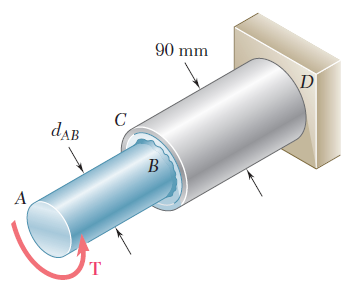
\includegraphics[width=0.35\textwidth]{img/p1.PNG}
\end{center}


\textbf{2.} Un eje sólido de acero ABC con 50 mm de diámetro es impulsado en
A por un motor que transmite 50 kW al eje a 10 Hz. Los engranes en B y C impulsan
maquinaria que requiere potencia igual a 35 kW y 15 kW, respectivamente.
Calcule el esfuerzo cortante máximo $\tau_{max}$ en el eje y el ángulo de torsión $\phi_{AC}$
entre el motor en A y el engrane en C. (Utilice G = 80 GPa). \puntos{30}

\begin{center}
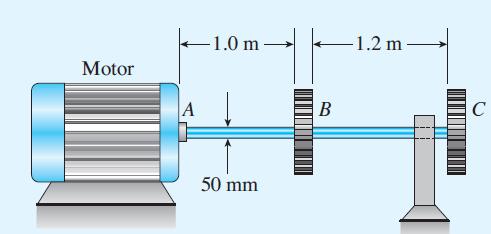
\includegraphics[width=0.45\textwidth]{img/p2.PNG}
\end{center}

\textbf{3.} Tres barras sólidas, cada una de 0.75 in de diámetro, están conectadas por engranes como 
se muestra en la figura. Sabiendo que $G=11.2x10^6 \text{ psi}$, calcule a) el ángulo que gira el extremo 
A del eje AB b) el ángulo que gira el extremo E del eje EF. \puntos{30}

\begin{center}
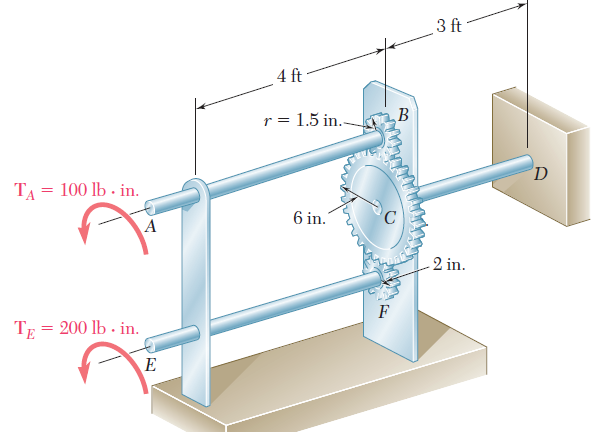
\includegraphics[width=0.45\textwidth]{img/p3.PNG}
\end{center}

\textbf{4.} Tipo de esfuerzo que presenta una barra circular sometida a pares de torsión. \puntos{5}

\begin{enumerate}[label=\alph*),itemsep=0pt]
\item Esfuerzo normal
\item Esfuerzo cortante
\item Esfuerzo de flexión
\end{enumerate}

\textbf{5.} Principales especificaciones que deben cumplirse en el diseño de un eje de transmisión. \puntos{5}

\begin{enumerate}[label=\alph*),itemsep=0pt]
\item Potencia a transmitir y velocidad de rotación del eje.
\item Torque a transmitir y condiciones de operación.
\item Diámetro robusto y bajas velocidades de rotación.
\end{enumerate}




\end{document}